\section{A path querying algorithm using conjunctive grammars}
In this section, we show how the path querying using conjunctive grammars and relational query semantics can be reduced to the calculation of the matrix transitive closure. We propose an algorithm that calculates the over-approximation of all conjunctive relations $R_A$, since the query evaluation using the relational query semantics and conjunctive grammars is undecidable problem~\cite{hellingsRelational}.

We define a \textit{conjunctive matrix multiplication}, $a \circ b = c$, where $a$ and $b$ are matrices of the suitable size that have subsets of $N$ as elements, as $c_{i,j} = \{A~|~\exists (A \rightarrow B_1 C_1~\& \ldots \&~B_m C_m) \in P \text{ such that } (B_k, C_k) \in d_{i,j} \}$, where $d_{i,j} = \bigcup^{n}_{k=1}{a_{i,k} \times b_{k,j}}$ and $(\times)$ is the Cartesian product. 

We define the \textit{conjunctive transitive closure} of a square matrix $a$ as $a^{conj} = a^{(1)} \cup a^{(2)} \cup \cdots$ where $a^{(i)} = a^{(i-1)} \cup (a^{(i-1)} \circ a^{(i-1)})$, $i \ge 2$ and $a^{(1)} = a$.

\subsection{Reducing conjunctive path querying to transitive closure} \label{section_reducing_conj}
In this section, we show how the over-approximation of all conjunctive relations $R_A$ can be calculated by computing the transitive closure $a^{conj}$.

Let $G = (N,\Sigma,P)$ be a conjunctive grammar and $D = (V, E)$ be a graph. We number the nodes of the graph $D$ from 0 to $(|V| - 1)$ and we associate the nodes with their numbers. We initialize $|V| \times |V|$ matrix $b$ with $\emptyset$. Further, for every $i$ and $j$ we set $b_{i,j} = \{A_k~|~((i,x,j) \in E) \wedge ((A_k \rightarrow x) \in P)\}$. Finally, we compute the conjunctive transitive closure $b^{conj} = b^{(1)} \cup b^{(2)} \cup \cdots$ where $b^{(i)} = b^{(i-1)} \cup (b^{(i-1)} \circ b^{(i-1)})$, $i \ge 2$ and $b^{(1)} = b$. For the conjunctive transitive closure $b^{conj}$, the following statements holds.

\begin{lemma}\label{lemma:conj}
	Let $D = (V,E)$ be a graph, let $G =(N,\Sigma,P)$ be a conjunctive grammar. Then for any $i, j$ and for any non-terminal $A \in N$, if $(i,j) \in R_A$ and $i \pi j$, such that there is a derivation tree according to the string $l(\pi)$ and a conjunctive grammar $G_A = (N,\Sigma,P,A)$ of the height $h \leq k$ then $A \in b^{(k)}_{i,j}$.
\end{lemma}
\begin{proof}(Proof by Induction)
	
	\textbf{Basis}: Show that the statement of the lemma holds for $k = 1$. For any $i, j$ and for any non-terminal $A \in N$, if $(i,j) \in R_A$ and $i \pi j$, such that there is a derivation tree according to the string $l(\pi)$ and a conjunctive grammar $G_A = (N,\Sigma,P,A)$ of the height $h \leq 1$ then there is edge $e$ from node $i$ to node $j$ and $(A \rightarrow x) \in P$ where $x = l(\pi)$. Therefore $A \in b^{(1)}_{i,j}$ and it has been shown that the statement of the lemma holds for $k = 1$.
	
	\textbf{Inductive step}: Assume that the statement of the lemma holds for any $k \leq (p - 1)$ and show that it also holds for $k = p$ where $p \geq 2$. Let $(i,j) \in R_A$ and $i \pi j$, such that there is a derivation tree according to the string $l(\pi)$ and a conjunctive grammar $G_A = (N,\Sigma,P,A)$ of the height $h \leq p$.
	
	Let $h < p$. Then by the inductive hypothesis $A \in b^{(p-1)}_{i,j}$. Since $b^{(p)} = b^{(p-1)} \cup (b^{(p-1)} \circ b^{(p-1)})$ then $A \in b^{(p)}_{i,j}$ and the statement of the lemma holds for $k = p$.
	
	Let $h = p$. Let $A \rightarrow B_1 C_1~\& \ldots \&~B_m C_m$ be the rule corresponding to the root of the derivation tree from the assumption of the lemma. Therefore the heights of all subtrees corresponding to non-terminals $B_1, C_1, \ldots B_m, C_m$ are less than $p$. Then by the inductive hypothesis $B_x \in b^{(p-1)}_{i,t_x}$ and $C_x \in b^{(p-1)}_{t_x,j}$, for $x = 1\ldots m$ and $t_x \in V$. Let $d$ be a matrix that have subsets of $N \times N$ as elements, where $d_{i,j} = \bigcup^{n}_{t=1}{b^{(p-1)}_{i,t} \times b^{(p-1)}_{t,j}}$. Therefore $(B_x, C_x) \in d_{i,j}$, for $x = 1\ldots m$. Since $b^{(p)} = b^{(p-1)} \cup (b^{(p-1)} \circ b^{(p-1)})$ and $(b^{(p-1)} \circ b^{(p-1)})_{i,j} = \{A~|~\exists (A \rightarrow B_1 C_1~\& \ldots \&~B_m C_m) \in P \text{ such that } (B_k, C_k) \in d_{i,j} \}$ then $A \in b^{(p)}_{i,j}$ and the statement of the lemma holds for $k = p$. This completes the proof of the lemma.
\end{proof}

\begin{mytheorem}\label{thm:correct_conj}
	Let $D = (V,E)$ be a graph and let $G =(N,\Sigma,P)$ be a conjunctive grammar. Then for any $i, j$ and for any non-terminal $A \in N$, if $(i,j) \in R_A$ then $A \in b^{conj}_{i,j}$.
\end{mytheorem}
\begin{proof}
	
	By the lemma~\ref{lemma:conj}, if $(i,j) \in R_A$ then $A \in b^{(k)}_{i,j}$ for some $k$, such that $i \pi j$ with a derivation tree according to the string $l(\pi)$ and a conjunctive grammar $G_A = (N,\Sigma,P,A)$ of the height $h \leq k$. Since the matrix $b^{conj} = b^{(1)} \cup b^{(2)} \cup \cdots$, then for any $i, j$ and for any non-terminal $A \in N$, if $A \in b^{(k)}_{i,j}$ for some $k \geq 1$ then  $A \in b^{conj}_{i,j}$. Therefore, if $(i,j) \in R_A$ then $A \in b^{conj}_{i,j}$. This completes the proof of the theorem.
\end{proof}

Thus, we show how the over-approximation of all conjunctive relations $R_A$ can be calculated by computing the conjunctive transitive closure $b^{conj}$ of the matrix $b$.



\subsection{The algorithm} \label{section_algorithm_conj}
In this section we introduce an algorithm for calculating the conjunctive transitive closure $b^{conj}$ which was discussed in Section~\ref{section_reducing_conj}.

The following algorithm takes on input a graph $D = (V, E)$ and a conjunctive grammar $G = (N,\Sigma,P)$.

\begin{algorithm}[H]
	\begin{algorithmic}[1]
		\caption{Conjunctive recognizer for graphs}
		\label{alg:graphParse_conj}
		\Function{conjunctiveGraphParsing}{D, G}
		
		\State{$n \gets$ a number of nodes in $D$}
		\State{$E \gets$ the directed edge-relation from $D$}
		\State{$P \gets$ a set of production rules in $G$}
		\State{$T \gets$ a matrix $n \times n$ in which each element is $\emptyset$}
		\ForAll{$(i,x,j) \in E$}
		\Comment{Matrix initialization}
		\State{$T_{i,j} \gets T_{i,j} \cup \{A~|~(A \rightarrow x) \in P \}$}
		\EndFor    
		\While{matrix $T$ is changing}
		
		\State{$T \gets T \cup (T \circ T)$}
		\Comment{Transitive closure calculation} 
		\EndWhile
		\State \Return $T$    
		\EndFunction
	\end{algorithmic}
\end{algorithm}

Similar to the case of the context-free grammars we can show that the Algorithm~\ref{alg:graphParse_conj} terminates in a finite number of steps. Since each element of the matrix $T$ contains no more than $|N|$ non-terminals, then total number of non-terminals in the matrix $T$ does not exceed $|V|^2|N|$. Therefore, the following theorem holds.

\begin{mytheorem}\label{thm:finite_conj}
	Let $D = (V,E)$ be a graph and let $G =(N,\Sigma,P)$ be a conjunctive grammar. Algorithm~\ref{alg:graphParse_conj} terminates in a finite number of steps. 
\end{mytheorem}
\begin{proof}
	It is sufficient to show, that the operation in line \textbf{9} of the Algorithm~\ref{alg:graphParse_conj} changes the matrix $T$ only finite number of times. Since this operation can only add non-terminals to some elements of the matrix $T$, but not remove them, it can change the matrix $T$ no more than $|V|^2|N|$ times.
\end{proof}

\subsection{An example}
In this section, we provide a step-by-step demonstration of the proposed algorithm for path querying using conjunctive grammars. The \textbf{example query} is based on the conjunctive grammar $G = (N, \Sigma, P)$ in binary normal form where:
\begin{itemize}
	\item The set of non-terminals $N = \{S, A, B, C, D\}$.
	\item The set of terminals $\Sigma = \{a, b, c\}.$
	\item The set of production rules $P$ is presented in Figure~\ref{ProductionRulesExampleQueryConj}.
\end{itemize}

\begin{figure}[h]
	\[
	\begin{array}{rccl}
	0: & S & \rightarrow & AB \ \& \ DC \\ 
	1: & A & \rightarrow & a \\ 
	2: & B & \rightarrow & BC \\ 
	3: & B & \rightarrow & b \\
	4: & C & \rightarrow & c \\ 
	5: & D & \rightarrow & AD \\ 
	6: & D & \rightarrow & b \\ 
	\end{array}
	\]
	\caption{Production rules for the conjunctive example query grammar.}
	\label{ProductionRulesExampleQueryConj}
\end{figure}

The conjunct $AB$ generates the language $L_{AB} = \{abc^*\}$ and the conjunct $DC$ generates the language $L_{DC} = \{a^*bc\}$. Thus, the language generated by the conjunctive grammar $G_S = (N, \Sigma, P, S)$ is $L(G_S) = L_{AB} \cap L_{DC} = \{abc\}$. We tun the query on a graph presented in Figure~\ref{conjExampleGraph}.

\begin{figure}[h]
	\[
	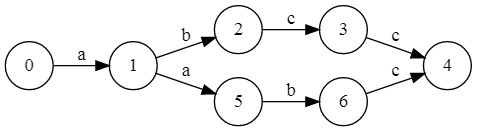
\includegraphics[width=0.8\textwidth]{pictures/ConjExampleGraph.png}
	\]
	\caption{An input graph for the conjunctive example query.}
	\label{conjExampleGraph}
\end{figure}

We provide a step-by-step demonstration of the work with the given graph $D$ and grammar $G$ of the Algorithm~\ref{alg:graphParse_conj}. After the matrix initialization in lines \textbf{6-7} of the Algorithm~\ref{alg:graphParse_conj}, we have a matrix $T_0$ presented in Figure~\ref{ConjExampleQueryInitMatrix}.

\begin{figure}[h]
	\[
	T_0 = \begin{pmatrix}
	\varnothing & \{A\} & \varnothing & \varnothing & \varnothing & \varnothing & \varnothing \\
	
	\varnothing & \varnothing & \{B, D\} & \varnothing & \varnothing & \{A\} & \varnothing \\
	
	\varnothing & \varnothing & \varnothing & \{C\} & \varnothing & \varnothing & \varnothing \\
	
	\varnothing & \varnothing & \varnothing & \varnothing & \{C\} & \varnothing & \varnothing \\
	
	\varnothing & \varnothing & \varnothing & \varnothing & \varnothing & \varnothing & \varnothing \\
	
	\varnothing & \varnothing & \varnothing & \varnothing & \varnothing & \varnothing & \{B, D\} \\
	
	\varnothing & \varnothing & \varnothing & \varnothing & \{C\} & \varnothing & \varnothing \\
	\end{pmatrix}
	\]
	\caption{The initial matrix for the example query.}
	\label{ConjExampleQueryInitMatrix}
\end{figure}

Let $T_i$ be the matrix $T$ obtained after executing the loop in lines \textbf{8-9} of the Algorithm~\ref{alg:graphParse_conj} $i$ times. To compute the matrix $T_1$ we need to compute the matrix $d$ where $d_{i,j} = \bigcup^{n}_{k=1}{T_{0_{i,k}} \times T_{0_{i,k}}}$. The matrix $d$ for the first loop iteration is presented in Figure~\ref{dmatrix}. The matrix $T_1 = $ $T_1 = T_0 \cup (T_0 \circ T_0)$ is shown in Figure~\ref{ConjExampleQueryFirstIteration}.

\begin{figure}[h]
	\noindent
	\resizebox{\linewidth}{!}{%
	$
	\begin{pmatrix}
	\varnothing & \varnothing & \{(A,B), (A,D)\} & \varnothing & \varnothing & \varnothing & \varnothing \\
	
	\varnothing & \varnothing & \varnothing & \{(B,C), (D,C)\} & \varnothing & \varnothing & \{(A,B), (A,D)\} \\
	
	\varnothing & \varnothing & \varnothing & \varnothing & \{(C,C)\} & \varnothing & \varnothing \\
	
	\varnothing & \varnothing & \varnothing & \varnothing & \varnothing & \varnothing & \varnothing \\
	
	\varnothing & \varnothing & \varnothing & \varnothing & \varnothing & \varnothing & \varnothing \\
	
	\varnothing & \varnothing & \varnothing & \varnothing & \{(B,C), (D,C)\} & \varnothing & \varnothing \\
	
	\varnothing & \varnothing & \varnothing & \varnothing & \varnothing & \varnothing & \varnothing \\
	\end{pmatrix}$%
	}
	\caption{The matrix $d$ for the first loop iteration.}
	\label{dmatrix}
\end{figure}

\begin{figure}[h]
	\[
	T_1 = \begin{pmatrix}
	\varnothing & \{A\} & \{D\} & \varnothing & \varnothing & \varnothing & \varnothing \\
	
	\varnothing & \varnothing & \{B, D\} & \{B\} & \varnothing & \{A\} & \{D\} \\
	
	\varnothing & \varnothing & \varnothing & \{C\} & \varnothing & \varnothing & \varnothing \\
	
	\varnothing & \varnothing & \varnothing & \varnothing & \{C\} & \varnothing & \varnothing \\
	
	\varnothing & \varnothing & \varnothing & \varnothing & \varnothing & \varnothing & \varnothing \\
	
	\varnothing & \varnothing & \varnothing & \varnothing & \{B\} & \varnothing & \{B, D\} \\
	
	\varnothing & \varnothing & \varnothing & \varnothing & \{C\} & \varnothing & \varnothing \\
	\end{pmatrix}
	\]
	\caption{The initial matrix for the example query.}
	\label{ConjExampleQueryFirstIteration}
\end{figure}

When the algorithm at some iteration finds new paths from the node $i$ to the node $j$ for all conjuncts of some production rule, then it adds nonterminal from the left side of this rule to the set $T_{i,j}$.

The calculation of the transitive closure is completed after $k$ iterations when a fixpoint is reached: $T_{k-1} = T_k$. For this example, $k = 4$ since $T_4 = T_3$. The remaining iterations of computing the transitive closure are presented in Figure~\ref{ConjExampleQueryFinalIterations}.

\begin{figure}
	\[
	T_2 = \begin{pmatrix}
	\varnothing & \{A\} & \{D\} & \{S\} & \varnothing & \varnothing & \{D\} \\
	
	\varnothing & \varnothing & \{B, D\} & \{B\} & \{S,B\} & \{A\} & \{D\} \\
	
	\varnothing & \varnothing & \varnothing & \{C\} & \varnothing & \varnothing & \varnothing \\
	
	\varnothing & \varnothing & \varnothing & \varnothing & \{C\} & \varnothing & \varnothing \\
	
	\varnothing & \varnothing & \varnothing & \varnothing & \varnothing & \varnothing & \varnothing \\
	
	\varnothing & \varnothing & \varnothing & \varnothing & \{B\} & \varnothing & \{B, D\} \\
	
	\varnothing & \varnothing & \varnothing & \varnothing & \{C\} & \varnothing & \varnothing \\
	\end{pmatrix}
	\]
	
	\[
	T_3 = \begin{pmatrix}
	\varnothing & \{A\} & \{D\} & \{S\} & \{S\} & \varnothing & \{D\} \\
	
	\varnothing & \varnothing & \{B, D\} & \{B\} & \{S,B\} & \{A\} & \{D\} \\
	
	\varnothing & \varnothing & \varnothing & \{C\} & \varnothing & \varnothing & \varnothing \\
	
	\varnothing & \varnothing & \varnothing & \varnothing & \{C\} & \varnothing & \varnothing \\
	
	\varnothing & \varnothing & \varnothing & \varnothing & \varnothing & \varnothing & \varnothing \\
	
	\varnothing & \varnothing & \varnothing & \varnothing & \{B\} & \varnothing & \{B, D\} \\
	
	\varnothing & \varnothing & \varnothing & \varnothing & \{C\} & \varnothing & \varnothing \\
	\end{pmatrix}
	\]
	
	\[
	T_4 = \begin{pmatrix}
	\varnothing & \{A\} & \{D\} & \{S\} & \{S\} & \varnothing & \{D\} \\
	
	\varnothing & \varnothing & \{B, D\} & \{B\} & \{S,B\} & \{A\} & \{D\} \\
	
	\varnothing & \varnothing & \varnothing & \{C\} & \varnothing & \varnothing & \varnothing \\
	
	\varnothing & \varnothing & \varnothing & \varnothing & \{C\} & \varnothing & \varnothing \\
	
	\varnothing & \varnothing & \varnothing & \varnothing & \varnothing & \varnothing & \varnothing \\
	
	\varnothing & \varnothing & \varnothing & \varnothing & \{B\} & \varnothing & \{B, D\} \\
	
	\varnothing & \varnothing & \varnothing & \varnothing & \{C\} & \varnothing & \varnothing \\
	\end{pmatrix}
	\]
	\caption{Remaining states of the matrix $T$.}
	\label{ConjExampleQueryFinalIterations}
\end{figure}

Thus, the result of the Algorithm~\ref{alg:graphParse_conj} for the example query is the matrix $T_4 = T_3$. Now, after constructing the transitive closure, we can construct the over-approximations $R'_A$ of the conjunctive relations $R_A$. These approximations for each non-terminal of the grammar $G$ are presented in Figure~\ref{ConjExampleQueryCFRelations}.

\begin{figure}
	\begin{eqnarray}
		R'_S&=&\{(0,3),(0,4),(1,4)\},\\
		R'_{A}&=&\{(0,1),(1,5)\},\\
		R'_{B}&=&\{(1,2),(1,3),(1,4),(5,4),(5,6)\}, \\
		R'_{C}&=&\{(2,3),(3,4),(6,4)\}, \\
		R'_{D}&=&\{(0,2),(0,6),(1,2),(1,6),(5,6)\}.
	\end{eqnarray}
	\caption{The over-approximations of the conjunctive relations for the example query.}
	\label{ConjExampleQueryCFRelations}
\end{figure}

This example demonstrates that it is not always possible to obtain an exact solution. For example, a pair of nodes $(0,4)$ belongs to $R'_S$, although there is no path from the node $0$ to the node $4$, which forms a string derived from the nonterminal $S$ (only the string $abc$ can be derived from the nonterminal $S$). Extra pairs of nodes are added if there are different paths from the node $i$ to the node $j$, which in summary correspond to all conjuncts of one production rule, but there is no path from the node $i$ to the node $j$, which at the same time would correspond to all conjuncts of this rule. For example, for the conjuncts of the rule $S \rightarrow AB \ \& \ DC$, there is a path from the node $0$ to the node $4$ forming the string $abcc$, and there is also a path from the node $0$ to the node $4$ forming the string $aabc$. The first path corresponds to the conjunct $AB$, since the string $abcc$ belongs to the language $L_{AB} = \{abc^*\}$, and the second path corresponds to the conjunct $DC$, since the string $aabc$ belongs to the language $L_{DC} = \{a^*bc\}$. However, it is obvious that there is no path from the node $0$ to the node $4$, which forms the string $abc$.
